% \documentclass[12pt]{article}

%%v helpful MIT exam schema, see http://www-math.mit.edu/~psh/exam/examdoc.pdf
 \documentclass[8pt]{exam} 
% \qformat{\textbf{Question \thequestion}\quad \thepoints\hfill } % Large depth to make space}
 \renewcommand{\thesubpart}{(\roman{subpart})}
 \renewcommand{\subpartlabel}{\thesubpart}
 \footer{}{}{Page \thepage\ de \numpages}
\addpoints
% \pointsinmargin
% \boxedpoints
\renewcommand{\questionshook}{\setlength{\itemsep}{0.2cm}}
\renewcommand{\partshook}{
	\setlength{\itemsep}{0.1cm}
}

\pagestyle{empty} %for handouts
\addtolength{\jot}{2em} % this makes all formulae a bit more spaced vertically for handouts
\setlength{\parindent}{0pt} %we're not writing a novel
%\renewcommand{\arraystretch}{2} %makes tables taller, so easier to write in

\usepackage[fleqn]{amsmath}
\usepackage{amssymb} %standard classy maths symbols
\usepackage[a4paper, margin=1in]{geometry} %makes it easy to specify where to put stuff on the page

\usepackage{siunitx} %v handy way of getting SI units to typeset correctly...
% \sisetup{locale = FR} %... and now it will use a comma for decimals

\usepackage[utf8]{inputenc}

% \usepackage[french]{babel} % frenchify everything (e.g. a Table becomes a Tableau)
% \usepackage{lmodern} % font with nicer French characters than standard
% \usepackage{textcomp} % and more help for special characters

\usepackage{tcolorbox} % basic but good package for boxes around text
\tcbset{colback=black!5!white}
% \usepackage{color} % colours
%\newcommand{\fillin}{\color{black!1!white}} %makes the text disappear
%\definecolor{fillin}{rgb} {1.00,1.00,1.00}
%\renewcommand{\fillin}{\color{blue}} \definecolor{fillin}{rgb} {0.00,0.00,1.00} %makes the filling in text appear (in blue)

\usepackage{enumitem} % can change the labels on lists, items, enumerates
\usepackage{setspace}

\usepackage{tikz, pgfplots} % interval diagrams, sets, etc.
\usetikzlibrary{calc,trees,positioning,arrows,fit,shapes}

\newcommand\TikCircle[1][2.5]{\tikz[baseline=-#1]{\draw[thick](0,0)circle(3mm)[radius=#1mm];}}

\begin{document}

\textbf{Name:} \dotfill (with calculator)

\



\begin{questions}


\question[2] 
Determine the co-ordinates of $P\big(\frac{5\pi}{6}\big)$ on the trigonometric circle below. \\ 
Give your answers as exact values.

\vspace{-5mm}
\begin{minipage}[t]{0.5\textwidth}
\fillwithdottedlines{42mm}
\end{minipage}
\begin{minipage}[t]{0.5\textwidth}
\vspace{0mm}
\begin{center}
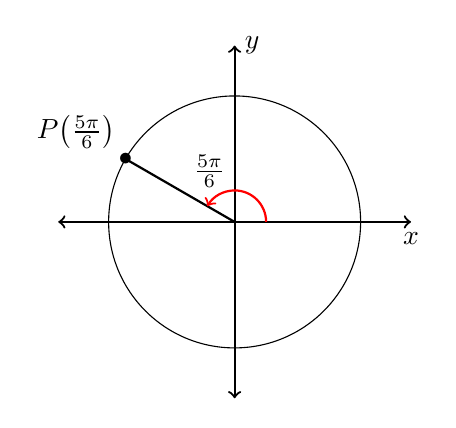
\begin{tikzpicture}[scale=0.8]
\draw (0,0) circle (2);
\draw[thick,<->] (0,-2.8) -- (0,2.8) node[right] {$y$}; 
\draw[thick,<->] (-2.8,0) -- (2.8,0) node[below] {$x$}; 

\draw[thick] (0,0) -- ({2*cos(150)},{2*sin(150)}) node {$\bullet$} node[above left] {$P\big(\frac{5\pi}{6}\big)$};
\draw[thick,red,->] (0.5,0) arc (0:150:0.5); 
\draw (-0.4,0.8) node {$\frac{5 \pi}{6}$};

\end{tikzpicture}
\end{center}
\end{minipage}

\vspace{-5mm}
\question[1] Give another angle $\alpha \neq \frac{5\pi}{6}$ such that $\sin(\alpha) = \sin(\frac{5\pi}{6})$.
\fillwithdottedlines{35mm}

\question[2] Find all solutions to the equation $\sin(\alpha) = \sin(\frac{5\pi}{6})$
\fillwithdottedlines{35mm}

\question[2] Factorize the quadratic in $\cos(t)$ to solve the equation $\cos^2(t) - 3\cos(t) + 2 = 0$ 
\fillwithdottedlines{35mm}




\vfill

\end{questions}

\begin{tcolorbox}

\textbf{Name of examiner:}

\begin{center}
\gradetable[h][questions]
\end{center}

\end{tcolorbox}


\end{document}